\documentclass[a4paper]{article}

% \usepackage[portuguese]{babel}
\usepackage[utf8]{inputenc}
\usepackage{amsmath}
\usepackage{graphicx}
\usepackage[colorinlistoftodos]{todonotes}
\providecommand{\keywords}[1]{\textbf{\textit{Index terms---}} #1}
\usepackage{appendix}
\usepackage{float}

\usepackage{tocloft}
\addtocontents{toc}{\cftpagenumbersoff{section}}
\usepackage{subfig}

\usepackage[final]{pdfpages}

\usepackage{listings}
\usepackage{fancyhdr}
\usepackage{hyperref}
\hypersetup{
        colorlinks,
        linkcolor={red!50!black},
        citecolor={blue!50!black},
        urlcolor={blue!80!black}
}

% todo:
% make index and links beautiful, maybe pnud5
% put bibliography
% include one or two images?
% review all
% make listings
% make zip with images of the cow
% see README.md and thesis again and dissertation
% send to Cristina, and gang of avatars
% send to VIRUS journal:
%   send in Vim printed PDF
%   send in HTML rendered and then PDF
%   send in Latex

\title{
Memory and dispersonification in social experiments:\\
anthropological physics and technoxamanic ebós
}
\author{Renato Fabbri}

\date{\today, version 0.1-beta}

\usepackage{etoolbox}

\makeatletter
\pretocmd{\chapter}{\addtocontents{toc}{\protect\addvspace{15\p@}}}{}{}
\pretocmd{\section}{\addtocontents{toc}{\protect\vspace{-3mm}}}{}{}
\makeatother


\begin{document}
\maketitle



\begin{abstract}
Both mythological and hacker histories have recognized roles for
dispersonification: it protects the messenger, facilitates the detachment
from the self-image, is an artistic technique, etc.  Brazil has an evident part
in this context, for it proclaims religious freedom since the colonization and
beforehand (through ecumenical natives), and holds a renowned and visceral hacker trace:
  the kludge culture (aka. 'cultura da gambiarra').  This article exposes this legacy by two
means: 1) the description of social experiments made by many participants at once;
2) memorials of images, videos, texts, music, webpages, groups,
avatars/nicks/pseudonyms, presentations, etc.  This text is itself an
experiment, and will be fed back to the community for comments before
publishing, as usual with any \emph{anthropological physics} experiment.  The
materials herein are no secret, and are usually unpublished, although most
of it is not bind to a DOI or an ISBN/ISSN.  Further directions are given as
seminal ideas because next steps will be given by the community upon diverse
interests and context stonework.
\end{abstract}

\keywords{
anthropological physics, technoxamanism, memorial, complex networks,
data mining
}

\tableofcontents

\section{What? or motivation}
The main motivation of what is described here was and is to enable
participants to take action in their networks by means of scientific
knowledge.  Such networks are complex and social topological
structures that are embedded in, and embed, other complex systems.  The ethic
issues that arise when experimenting with other humans are ameliorated by following
\emph{anthropological physics}~\cite{anPhy,anPhy2,thesis} guidelines:
researchers or activists should keep the endeavors as open as possible (texts,
software, data, processes, outcomes, people involved, etc) while studying and
experimenting in their own networks; a trace inherited from ethnography and
similar to the technique/strategy of writing diaries.

\begin{figure}[!h]
  \centering
    \subfloat{\includegraphics[width=0.5\textwidth]{acervo/vaquinha/FASE1/CoolmeiaAmizades__}}
    \subfloat{\includegraphics[width=0.5\textwidth]{acervo/vaquinha/FASE1/CoolmeiaAmizadesNomes}}
  \caption{Friendship network of the Facebook Group called Hive (aka. \emph{Coolmeia} in Portuguese), with and without the names of the participants. Each node is a participant, each link is a friendship.}
\end{figure}

\section{How? or social, technoxamanic experiments of Collection and Diffusion of information}
Many experiments were carried out by diverse human agents, either directly or
through a second/fake/pseudonym/avatar/nick profile, i.e. people, for various
reasons, made conscious efforts in order to interact with their networks to
achieve specific goals or inspect the outcome.  Two examples are very efficient
in exposing the procedures and potentials: one that is continuous within few
months, another that is ephemeral and occurs in only a few hours or less.  In such
a diversity-rich setting, these experimental procedures were called
\emph{technoxamanic experiments} aka.  {\bf ebós}.

\begin{figure}[!h]
  \centering
    \subfloat{\includegraphics[width=0.5\textwidth]{acervo/vaquinha/FASE1/CienciasComFronteiras}}
    \subfloat{\includegraphics[width=0.5\textwidth]{acervo/vaquinha/FASE1/CienciasComFronteiras_nomes}}
  \caption{Friendship network of the Facebook Group called 'Cience with Frotiers' (aka. \emph{Ciências Com Fronteiras} a pun with the Cience without Frontiers Brazilian federal program), with and without the names of the participants.}
\end{figure}



\subsection{the Cow of the End of the World (continuous experiment):
progressive network activation from Peripherals to Hubs for a crowdfunding}\label{cont}

This is maybe the most powerful mechanism by which we performed collection and diffusion of information.
The results were very effective in spreading information about social networks,
in gathering knowledge from diverse parties and in modifying the social structures
in which I participate.
Most concretely, academics came to São Carlos for formal meetings,
new collaborations were established (such a UNDP grant were the Brazilian Presidency signed as beneficiary,
as described in the Appendix C of~\cite{thesis}),
money was obtained (various contributors transferred a total of about 3000 Brazilian Reais)
and my Facebook network increased about 50\% with individuals interested in the research.
The process consisted in:
\begin{enumerate}
	\item Downloading my Facebook friendship network. This was done by means of the Netvizz software,
		which is not possible nowadays and requires scrapping of Facebook pages because of new usage terms.
	\item Sorting my friends from the less connected to the more connected, i.e. from my friends that have less friends in common with me to the ones that have more friends in common; i.e. from periphery to hubs.
	\item Sending private messages for each of my friends, in such order.
		The messages were derived from a template I conceived in which I exposed the research and the information diffusion process.
	\item Making steps 1-3 for three times.
\end{enumerate}
In each cycle of steps 1-3, my friendship network grew about 15\% and there were typical reactions in each cycle.
In the first cycle, estrangement was ubiquitous and the replies were e.g. ``what are these network structures?'',
``what are you doing? I can't understand!'', ``I never though of such a thing as these networks''.
In the second cycle, they replied with interest and support.
In the third cycle, they engaged in establishing collaborations with visits, in the elaboration of documents and technologies and
in co-working proposals.

The data related to these three cycles can be downloaded in the personal data Facebook interface, and then analysed.
The experiment was carried in scientific terms and initial hypothesis were confirmed by these results.
Even so, these results are not still confirmed by performing the experiment again,
which poses both a problem and a potential scientific undertake.
Given that the diffusion process was done in Dec/2012-Jan/2013, it was frequently considered by fellow specialists as
having some influence in the civil society mobilization that occurred in Brazil in Mar/2013 and thereafter.
A very simple PDF document was built afterwards for delivering back these results to the networks~\cite{docDif}.

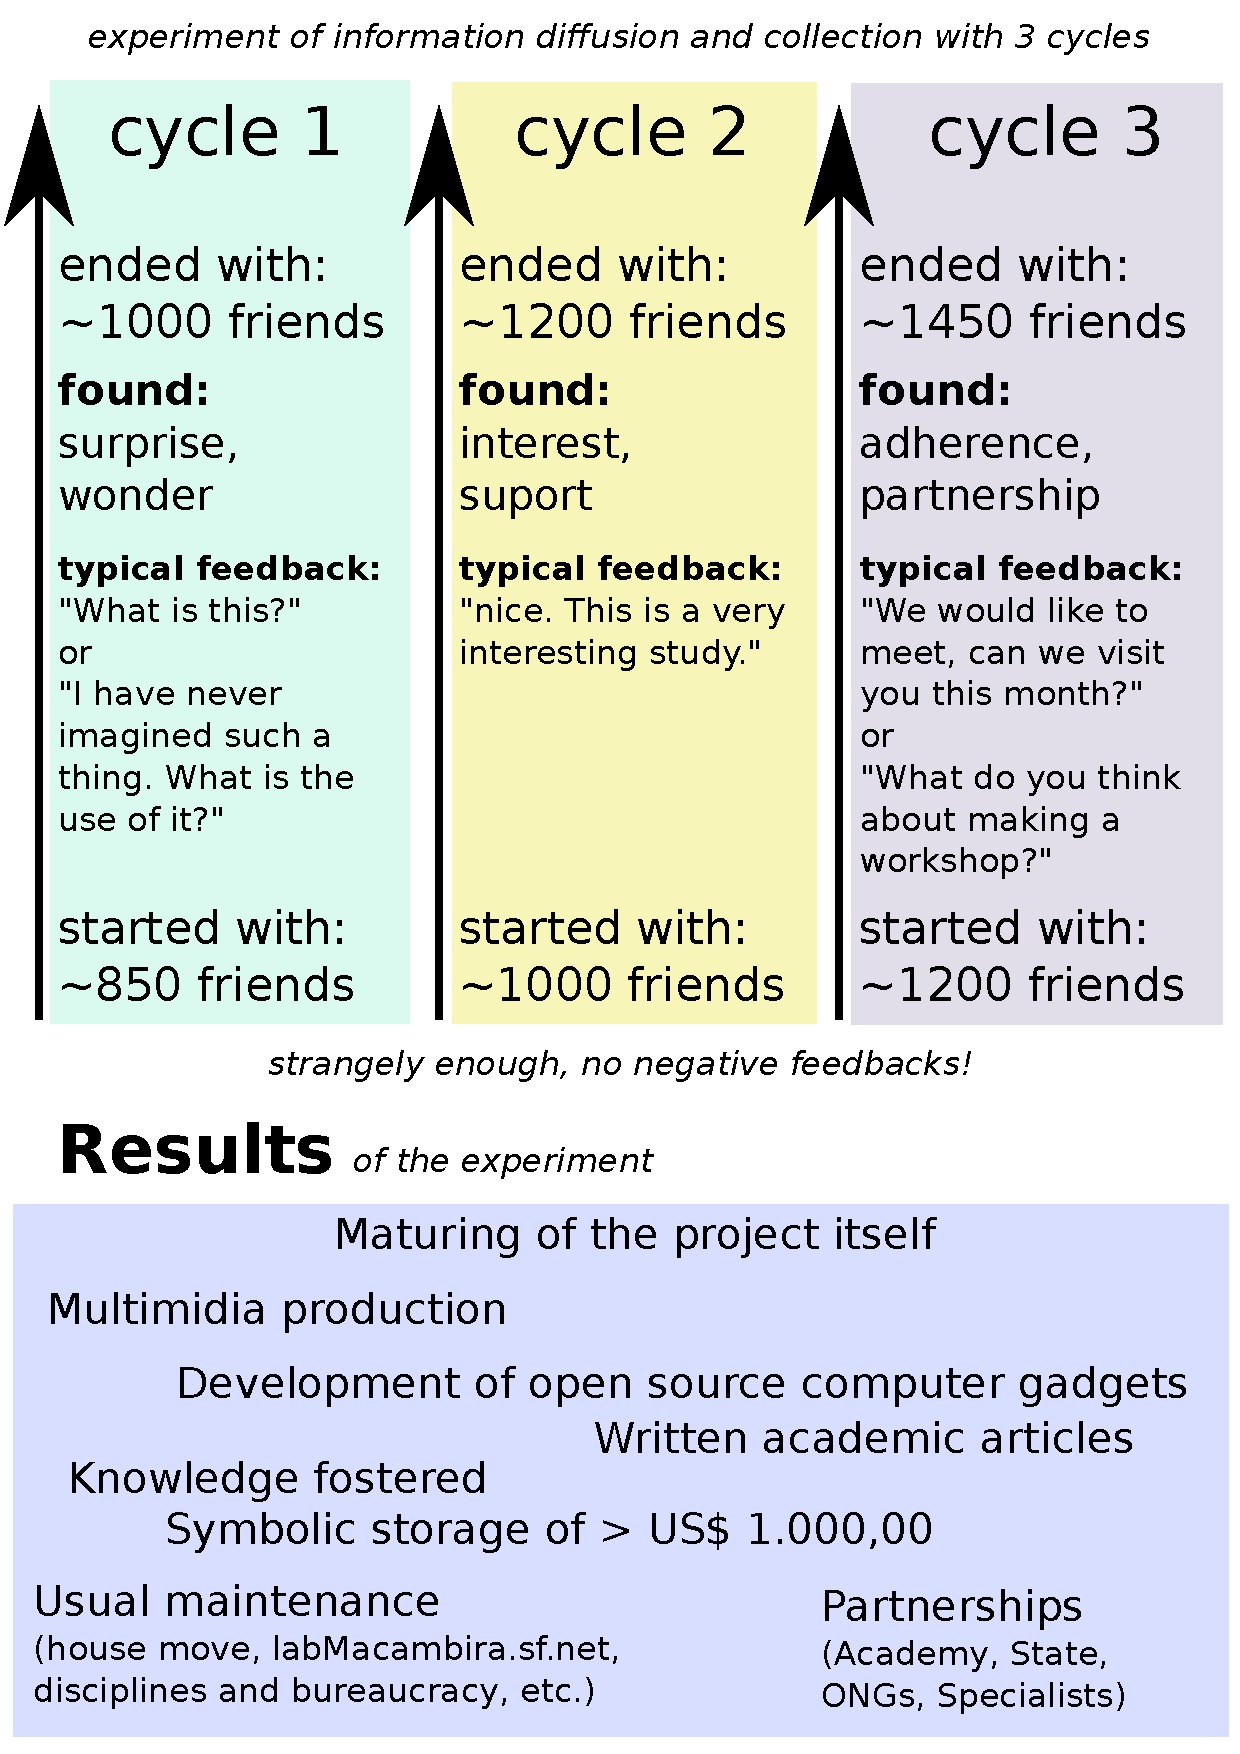
\includepdf{progressiveDiffusion.pdf}

\subsection{Betweenness VS Closeness centralities (ephemeral experiment)}~\label{eph}
This was first thought about in meetings with the artist and activist Pedro Paulo Rocha.
The idea was to activate the network not by means of a longstanding process such
as described in the last section, but by an ephemeral endeavor.
There were some artistic performances with this proposal, in which I did
not participate.
Nevertheless, there was one of these instantaneous activation processes that
I have done in conjunction with other specialists which was rather interesting.
In analyzing Facebook ego friendship networks, I fount that the set of $\approx 50$ members with
the greatest betweenness centrality was disjoint with the set of $\approx 50$ members
with the greatest closeness centrality, which is very unexpected.
Therefore I proposed that one should send the same message to both set of friends separately.
The messages were different for each person performing the experiment,
and it was about something they were interested in and wanted to spread and get feedback.
The result was systematic: the set of friends with greatest betweenness always reacted very friendly
with encouraging messages and sharing the original message in their timelines.
The set of friends with greatest closeness always reacted with many leaving the chat group
and with no replies.
We hypothesize that these reactions are because the large betweenness set of friends is more
likely to have control over the information flowing in the corresponding ego network while
the large closeness set of friends is more likely to observe/receive influence by the information.
This experiment was performed by partners related to the consulting reported in Section~\ref{cont}
and other partners involved in making an international technoxamanic festival.

A couple of years after these experiments, I made some visualizations to confirm or refute
that the highest closeness and betweenness are not the same participants.
The result was rather interesting: they were the same.
So either the Gephi algorithm used in 2014 is distinct from the one used by
NetworkX (in 2017) or something was done wrong, such as a human error or a bug,
or the networks analyzed in 2014 were very distinct from all the networks analyzed in 2017.
Figure~\ref{nh} exposes this contradiction with previously found results.

\begin{figure}[H]
  \centering
    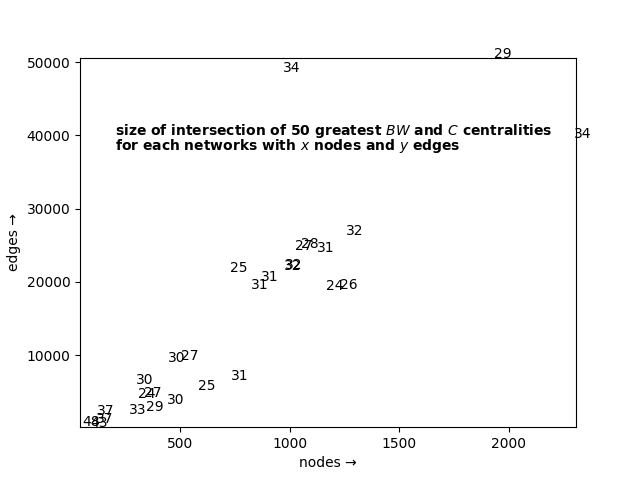
\includegraphics[width=0.9\textwidth]{netHip}
  \caption{An empirical evidence that the sets of participants with greatest betweennees ($BW$) and closeness ($C$) centralities are not as distinct as reported in the experiment described in Section~\ref{eph}.}\label{nh}
\end{figure}

\subsection{massive tagging and cross-posting (semi-ephemeral experiment)}\label{mass}
One very simple process by which collection and diffusion of information is being performed
is by tagging many friends in Facebook posts.
Currently, one can tag up to 100 friends in a post
and we did not find any limit for tagging friends in comments.
If one makes abusive use of tagging (too many posts or too many comments)
the Facebook platform sometimes restricts the permissions of that user.
Even so, I have made many posts with up to 100 friends tagged and tagged more
friends in the comments and made experiments such as the ones described in the
last sections and never got restricted.
It seems that the platform has some automated behavior but employees actually
perform the restrictions at least in some cases.
The employees might check the posts, tagging and messages to see if it is
really spam or in anyway abusive.
In~\cite{anExp} are some notes and data of one of these experiments (and a preliminary script for analysis).
The \emph{anthropological physics} guidelines~\cite{anPhy,anPhy2} probably prevented
these open, collective and scientific experiments from getting restrictions.
This hypothesis should be verified through direct contact with Facebook data scientists,
or by further testing the platform.
Figure~\ref{massive} illustrates the citation of Facebook participants in a massive tagging experiments.

\begin{figure}[H]
  \centering
    
\includegraphics[width=0.7\textwidth]{Screenshot}
  \caption{A screenshot of the tagged names is one of the massive tagging experiments reported in Section~\ref{mass}. Often, apart from citation of users in comments, the post also had the maximum number of 100 friends tagged.}\label{massive}
\end{figure}

Another powerful way by which many times diffusion and collection (of information?) is performed
is by crossposting, i.e. by sending a message to many email lists
at the same time.
Most participants find crossposting (very) effective but email list users also (rarely) report understanding such practice as abusive.
E.g. no one sent (me) a message reporting discomfort with (my) crossposts.
There was one occasion some years ago when a user replied with a challenge for
arguing why the crosspost what appropriate and then made some good contributions.
I personally perceive that this prejudice against crosspost is one of the main reasons
why email groups are losing users to other communication protocols such as provided by
Facebook, Whatsapp, Telegram and Diaspora.

\subsection{video-conferences, etherpads, websites, gadgets, and whatnot}\label{video}
Trivial, but relevant to notice here that periodic meetings are often held
(for diverse purposes and within arbitrary (social and technological) protocols.
Texts are yield by many writers at the same time using e.g. Etherpads (and Google Docs, but less frequent).
Websites and numerous software gadgets~\cite{ttmRepos} were used to make content and routines
freely available. All these resources are described in the Appendix C of~\cite{thesis}.
      
\section{so What and How? or the outcomes}
Section~\ref{cont} describes a procedure that resulted in
relevant professional, personal and financial achievements.
Sections~\ref{eph}-\ref{video} are directly linked to cultural identity and effervescence.
Next section mentions the media legacy entailed.

\section{What by Whom? or galleries / memorial}
Many of the agents are listed in Appendix~\ref{avatar}.
Posts with many tagged people (100 at most, although citing friends in comments is less restricted in Facebook)) are in Appendix~\ref{posts}.
Websites, groups, videos, image galleries, texts, music, ontologies and vocabularies, are all in the listings of the Appendixes.

\begin{figure}[!h]
  \centering
    \includegraphics[width=\textwidth]{acervo/vaquinha/FASE1/Larissa20022013}
  \caption{Friendship ego network of the visual artist Larissa Anzoategui. She is not on the network, but all her friends are.}
\end{figure}

\section{What shall we remember? or Memory and Narrative}
In fact, the social participation ontologies and vocabularies in~\cite{thesis}
are being worked on only (or mostly) academically.
There have been no evidence that the UN or the Brazilian Presidency are using
such formalized conceptualizations for discussions or to link and make available State-related data.
The Nexos (interdisciplinary research) group is very active nationwide,
and have provided insights grounded on the \emph{critical theory} tradition~\cite{anPhy2,thesis}.
The narrative of opening our State, Government, and Civil Society structures
and mannerisms has raised in scope, which is the core improvement of all
the efforts exposed in this document.
Next steps might be taken in the direction of minimizing imprecision
in personal and institutional data,
potentially though DLT (e.g. blockchain) and Linked Data/Semantic Web.

\begin{figure}[!h]
  \centering
    \includegraphics[width=\textwidth]{acervo/vaquinha/FASE2/Massimo}
  \caption{Friendship ego of the anthropologist Massimo Canevacci. He is not in the network, but all this friends are.}
\end{figure}

\subsection{A word about restriction of access and privacy}
Our social networking platforms are not optimized for indexing activity
and found resources.
This adds to a deficient use of our own social structures,
of our own private and public data.
Participatory democracy (e.g. liquid democracy) becomes less prominent,
private messages are valued in prejudice of open communication.

\begin{figure}[!h]
  \centering
    \hbox{\hspace{1.5em} \includegraphics[width=\textwidth]{acervo/vaquinha/FASE1/PracaPopular_interacoes_nomes}}
  \caption{Interaction network of the Facebook Group called 'Populare Park' (aka. \emph{Praça Popular} in Portuguese.}
\end{figure}

\begin{thebibliography}{9}
\bibitem{anPhy}
	Fabbri, R. \textbf{What are you and I?} [anthropological physics fundamentals], 2015. Available at \url{https://www.academia.edu/10356773/What\_are\_you\_and\_I\_anthropological\_physics\_fundamentals\_}

\bibitem{anPhy2}
	Fabbri, R.; Pisani, M.; Antunes, D. \textbf{Anthropological physics and social psychology in the critical research of networks}. Complex Networks Digital Campus (CS-DC'15).
	Em \\\url{http://cs-dc-15.org/papers/cognition/social-psychology/anthropological-physics-and-social-psychology-in-the-critical-research-of-networks/}

\bibitem{thesis}
Fabbri, R. (2017). \textbf{Topological stability and textual differentiation in human interaction networks:}
		statistical analysis, visualization and linked data. Doctoral thesis.
		From \url{https://github.com/ttm/thesis/raw/master/thesis-rfabbri.pdf}

\bibitem{docDif}
	Fabbri, R. \textbf{A document reporting the progressive diffusion of information from peripherals to hubs}. 2013. Available from: \url{https://dl.dropboxusercontent.com/u/22209842/doc/mit/progressiveDiffusion.pdf}. Accessible at: 15 Mar. 2017.

\bibitem{anExp}
	Fabbri, R. \textbf{Notes, data and a preliminary analysis script of a massive Facebook tagging social experiment}. 2015. Available from: \url{https://github.com/ttm/anthropologicalExperiments}. Accessible at: 15 Mar. 2017.

\bibitem{ttmRepos}
	Fabbri, R. \textbf{Various software gadgets}. 2012-2018. Available from: \url{https://github.com/ttm/}. Accessible at: 10 May. 2018.

\end{thebibliography}

\clearpage
\addtocontents{toc}{\protect\vskip.35cm} 
\begin{appendices}
{\Large \bf Appendixes}
\\

This appendix holds a memorial through short contextualizations
and listings.
Following the \emph{anthropological physics} guidelines to ameliorate
ethic issues, the materials are as related to the author as possible,
considering the reasons and relevance of the exposition.

  \begin{figure}[!h]
  \centering
    \subfloat{\includegraphics[width=0.52\textwidth]{acervo/vaquinha/FASE1/LeiCulturaViva50_Outra}}
    \subfloat{\includegraphics[width=0.4577\textwidth]{acervo/vaquinha/FASE1/LeiCulturaViva_Outra2_nomes}}
  \caption{Bipartite interaction network of posts and participants of the Facebook Group called 'Alive Culture' (aka. \emph{Cultura Viva} in Portuguese. Each node is either a post or a participant, each link is an interaction (i.e. a comment or reaction such as like).}
\end{figure}

\section{avatars/nicks/pseudonyms}\label{avatar}
\section{websites}
\section{posts}\label{posts}
\section{groups}
labmacambira, metareciclagem, submidialogia, tecnomagias
grupos do fb
canais de irc
\section{videos}
\section{image galleries}
\section{texts}
nuvens cognitivas
tese e dissertacao
\section{musical pieces}
half shape
\section{ontologies and vocabularies}
\end{appendices}


\end{document}


